\thispagestyle{plain}
\chapter{Evaluation}

This chapter covers the experiments that we conducted to compare our partitioning algorithms to the state-of-the-art. We will briefly go over the setup and the software parameters that were used for the experiments in Section \ref{sec:setup}. Then we cover the datasets and workloads on which the experiments were evaluated in Section \ref{sec:datasets}. Finally, we present the results of the partitioning algorithms and benchmarks in Sections \ref{sec:respartitions} and \ref{sec:resperformance}.

\section{Setup}\label{sec:setup}
All benchmarking experiments were conducted on a server with //TODO: hardware.

As index configuration parameters we chose the following:
//TODO: insert parameters


\section{Datasets and Workloads}\label{sec:datasets}

To evaluate our partitioning algorithms we chose to look at a variety of datasets and workloads to get a good understanding of how our partitioning algorithms work in practice. As for the datasets, we chose to use synthetic as well as real-world representatives to first see how the algorithms perform on pure datsets with a clear distribution and then see if the algorithms translate well to irregular patterns in real-world data. All datasets consist of 64-bit unsigned integers.

Figure \ref{fig:cdfs} shows the cumulative distribution function (CDF) of the keys in different datasets that were used throughout the experiments. In the top row, the left graph show the CDF of dense, uniformly distributed keys in the range of 0 to 100 million. Naturally, it corresponds to a simple linear function. The middle graph displays the same for the real-world \verb|osm| dataset. We can see that there are many keys located around $0.5 \cdot 10^{19}$ and $1.0 \cdot 10^{19}$, which corresponds to the jumps at these points in the CDF. The third CDF shows the distribution of the real-world \verb|fb| dataset. The particular shape of the CDF here is caused by large outliers in the key domain. In the second row, we see CDF of the real-world datasets \verb|books| and \verb|wiki|. The real-world datasets are taken from \citeauthor{Kipf2019} \cite{Kipf2019}. \verb|osm| contains uniformly sampled OpenStreetMap locations represented by their Cell IDs, \verb|fb| is a version of a Facebook user ID dataset, \verb|books| is a dataset of book sale popularity and \verb|wiki| contains Wikipedia article edit timestamps. Each of them consists of 200 million keys.

\begin{figure}
    \centering
    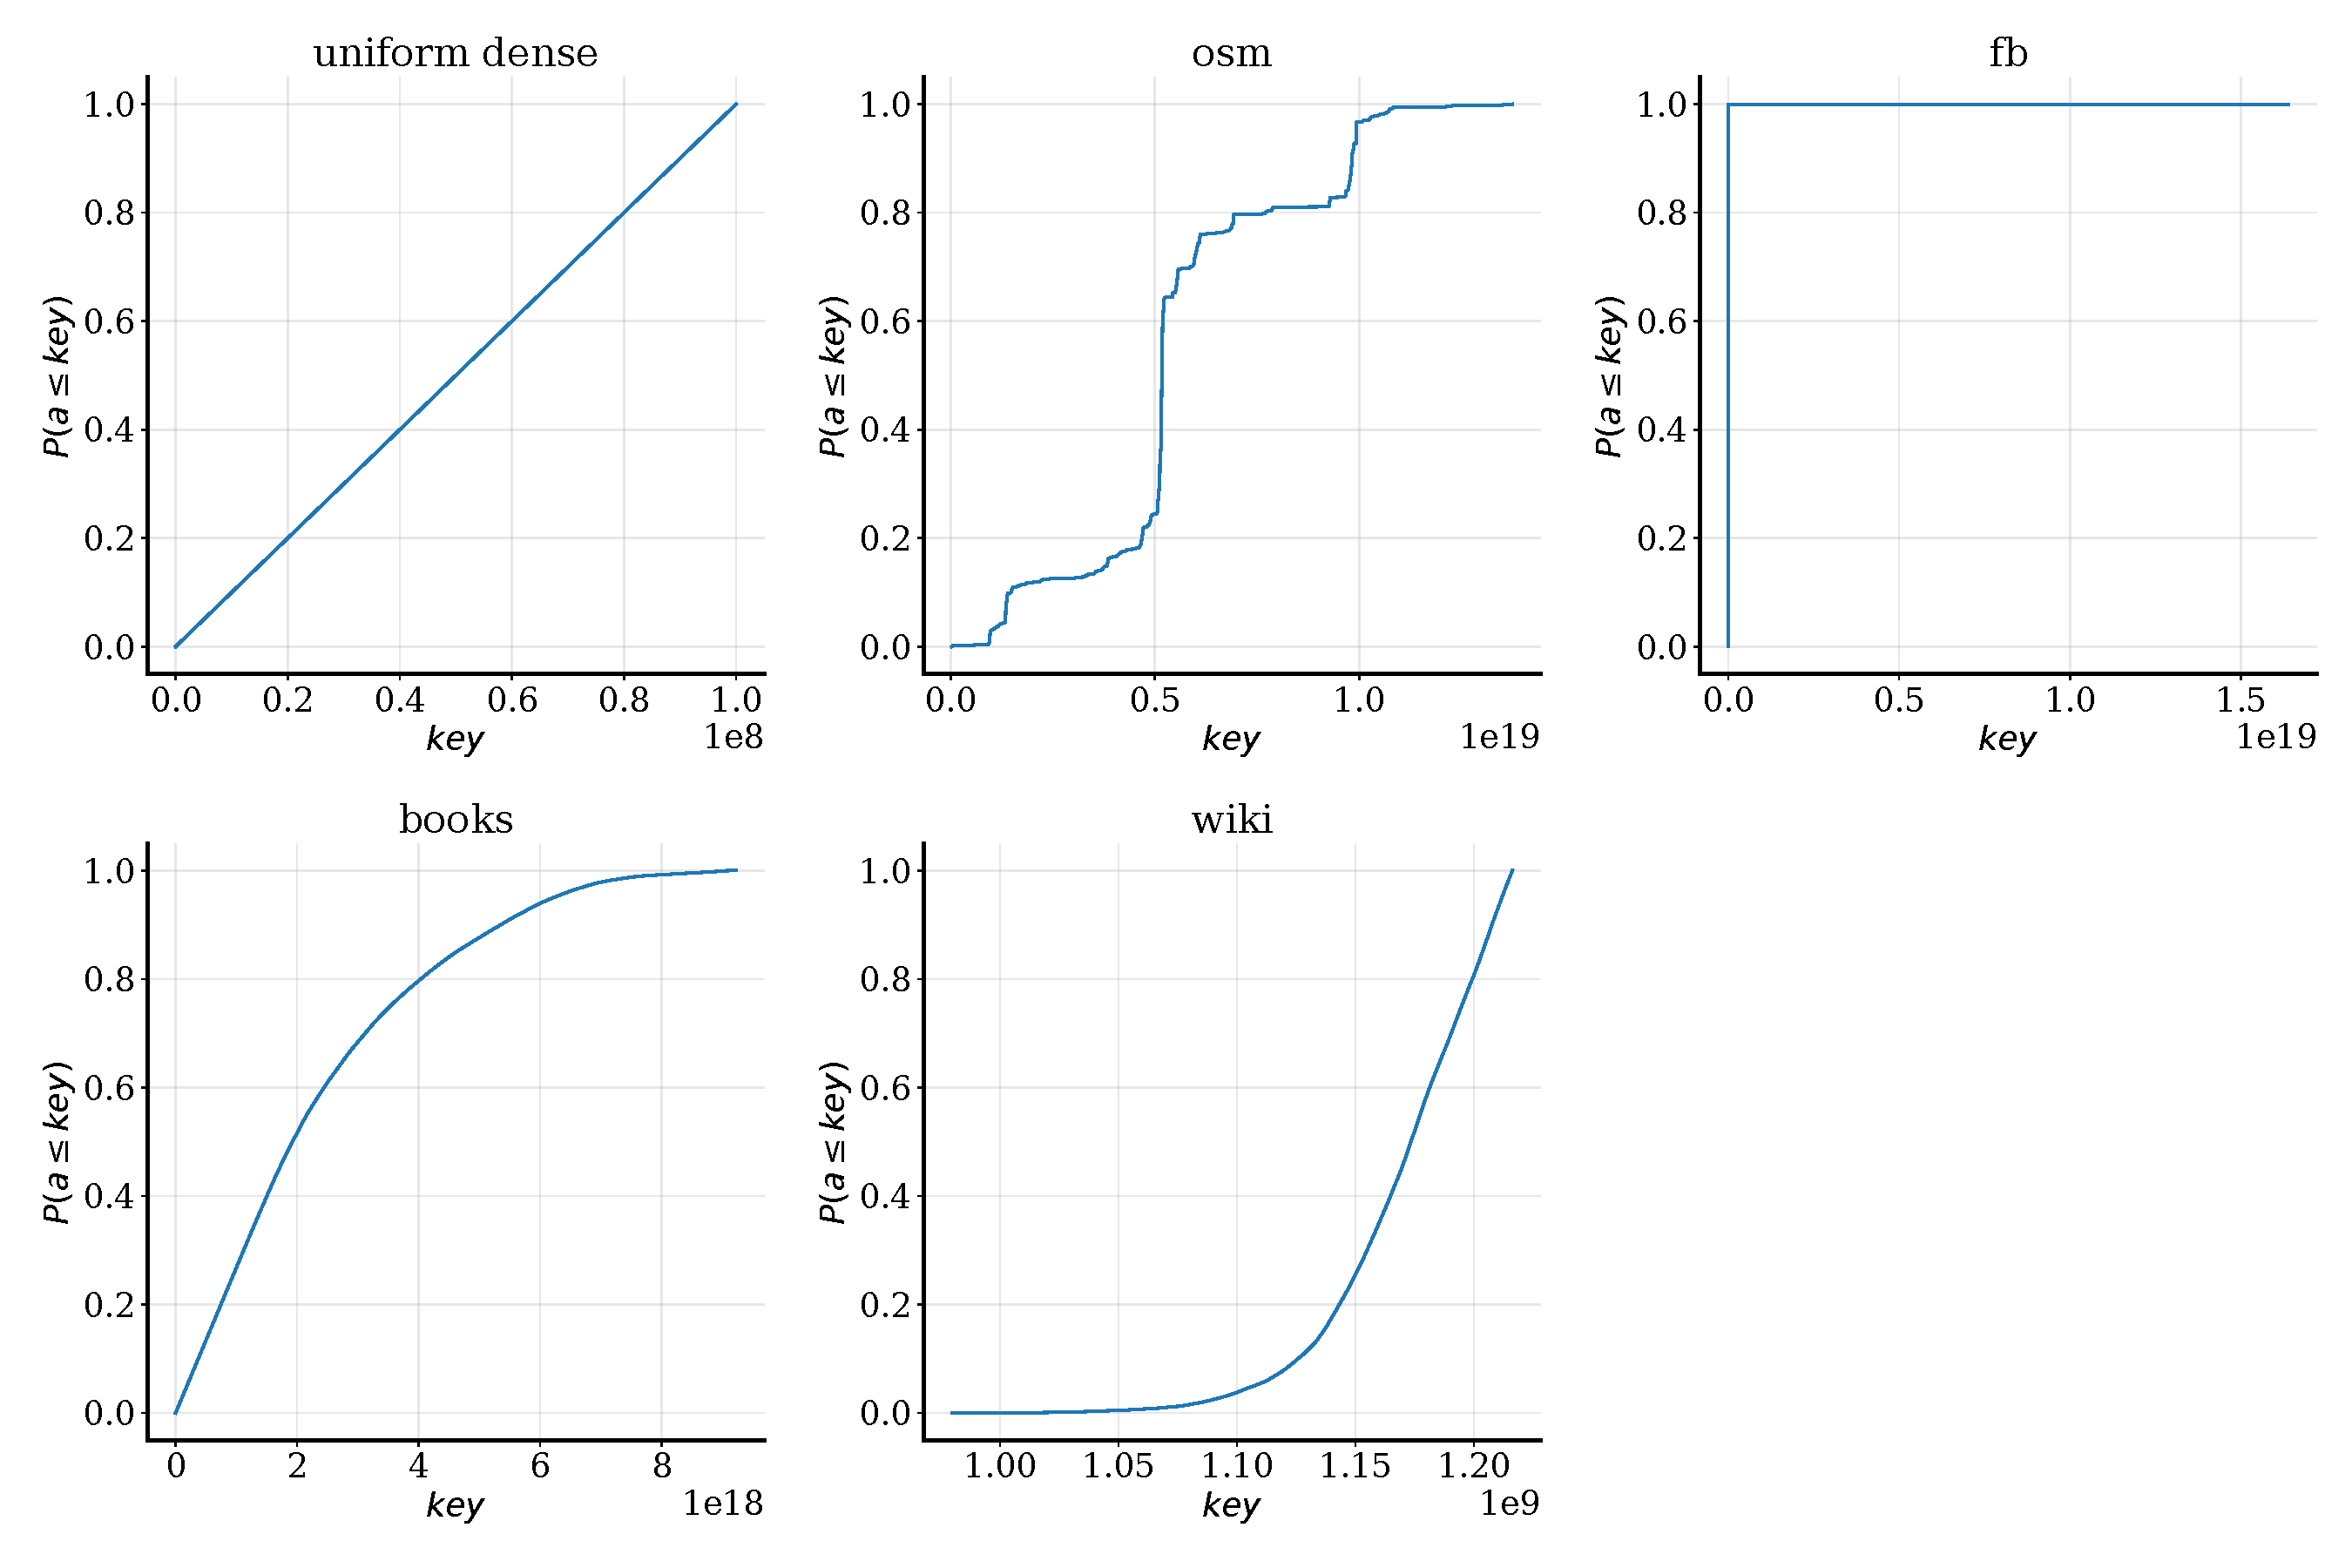
\includegraphics[width=\textwidth]{figures/cdfs.pdf}
    \caption{Cumulative Distribution Function of different datasets}
    \label{fig:cdfs}
\end{figure}

For the workloads, we proceed according to the generation described in Section \ref{sec:wklgeneration}. As an example, Listing \ref{lst:generation} shows the code that would be used to generate a bimodal distribution of point queries. This is simply achieved by overlapping the two specified regions such that the two normal distributions form a bimodal distribution. The overlap is achieved by specifying the \verb|min| and \verb|max| attributes such that the \verb|max| of the first distribution is greater than the \verb|min| of the second distribution. In this case, the first normal distribution covers the first 70\% of the keys and the second distribution covers the last 70\% of the keys. The 40\% of the keys in the middle will receive queries generated from both the first and the second distribution. The corresponding query distribution can be seen in Figure \ref{fig:bimodal}. Of course, the query distribution is dependent on the data distribution it is applied to. While the data distribution in the first row was a uniform one to show the shape of the query distribution, the second row shows the same query distribution when sampling from data that is exponentially distributed.

\begin{lstlisting}[language=Python, caption=Example workload generation from Region objects, label=lst:generation]
    regions = [
        Region(
            qtype=QueryType.POINT, 
            num=100000, 
            distribution=DistributionType.NORMAL, 
            index=True, 
            min=0, 
            max=0.7*len(data)
        ),
        Region(
            qtype=QueryType.POINT, 
            num=100000, 
            distribution=DistributionType.NORMAL, 
            index=True, 
            min=0.7*len(data), 
            max=len(data)
        )
    ]
    wkl = Workload.from_regions(data, regions)
\end{lstlisting}

\begin{figure}
    \centering
    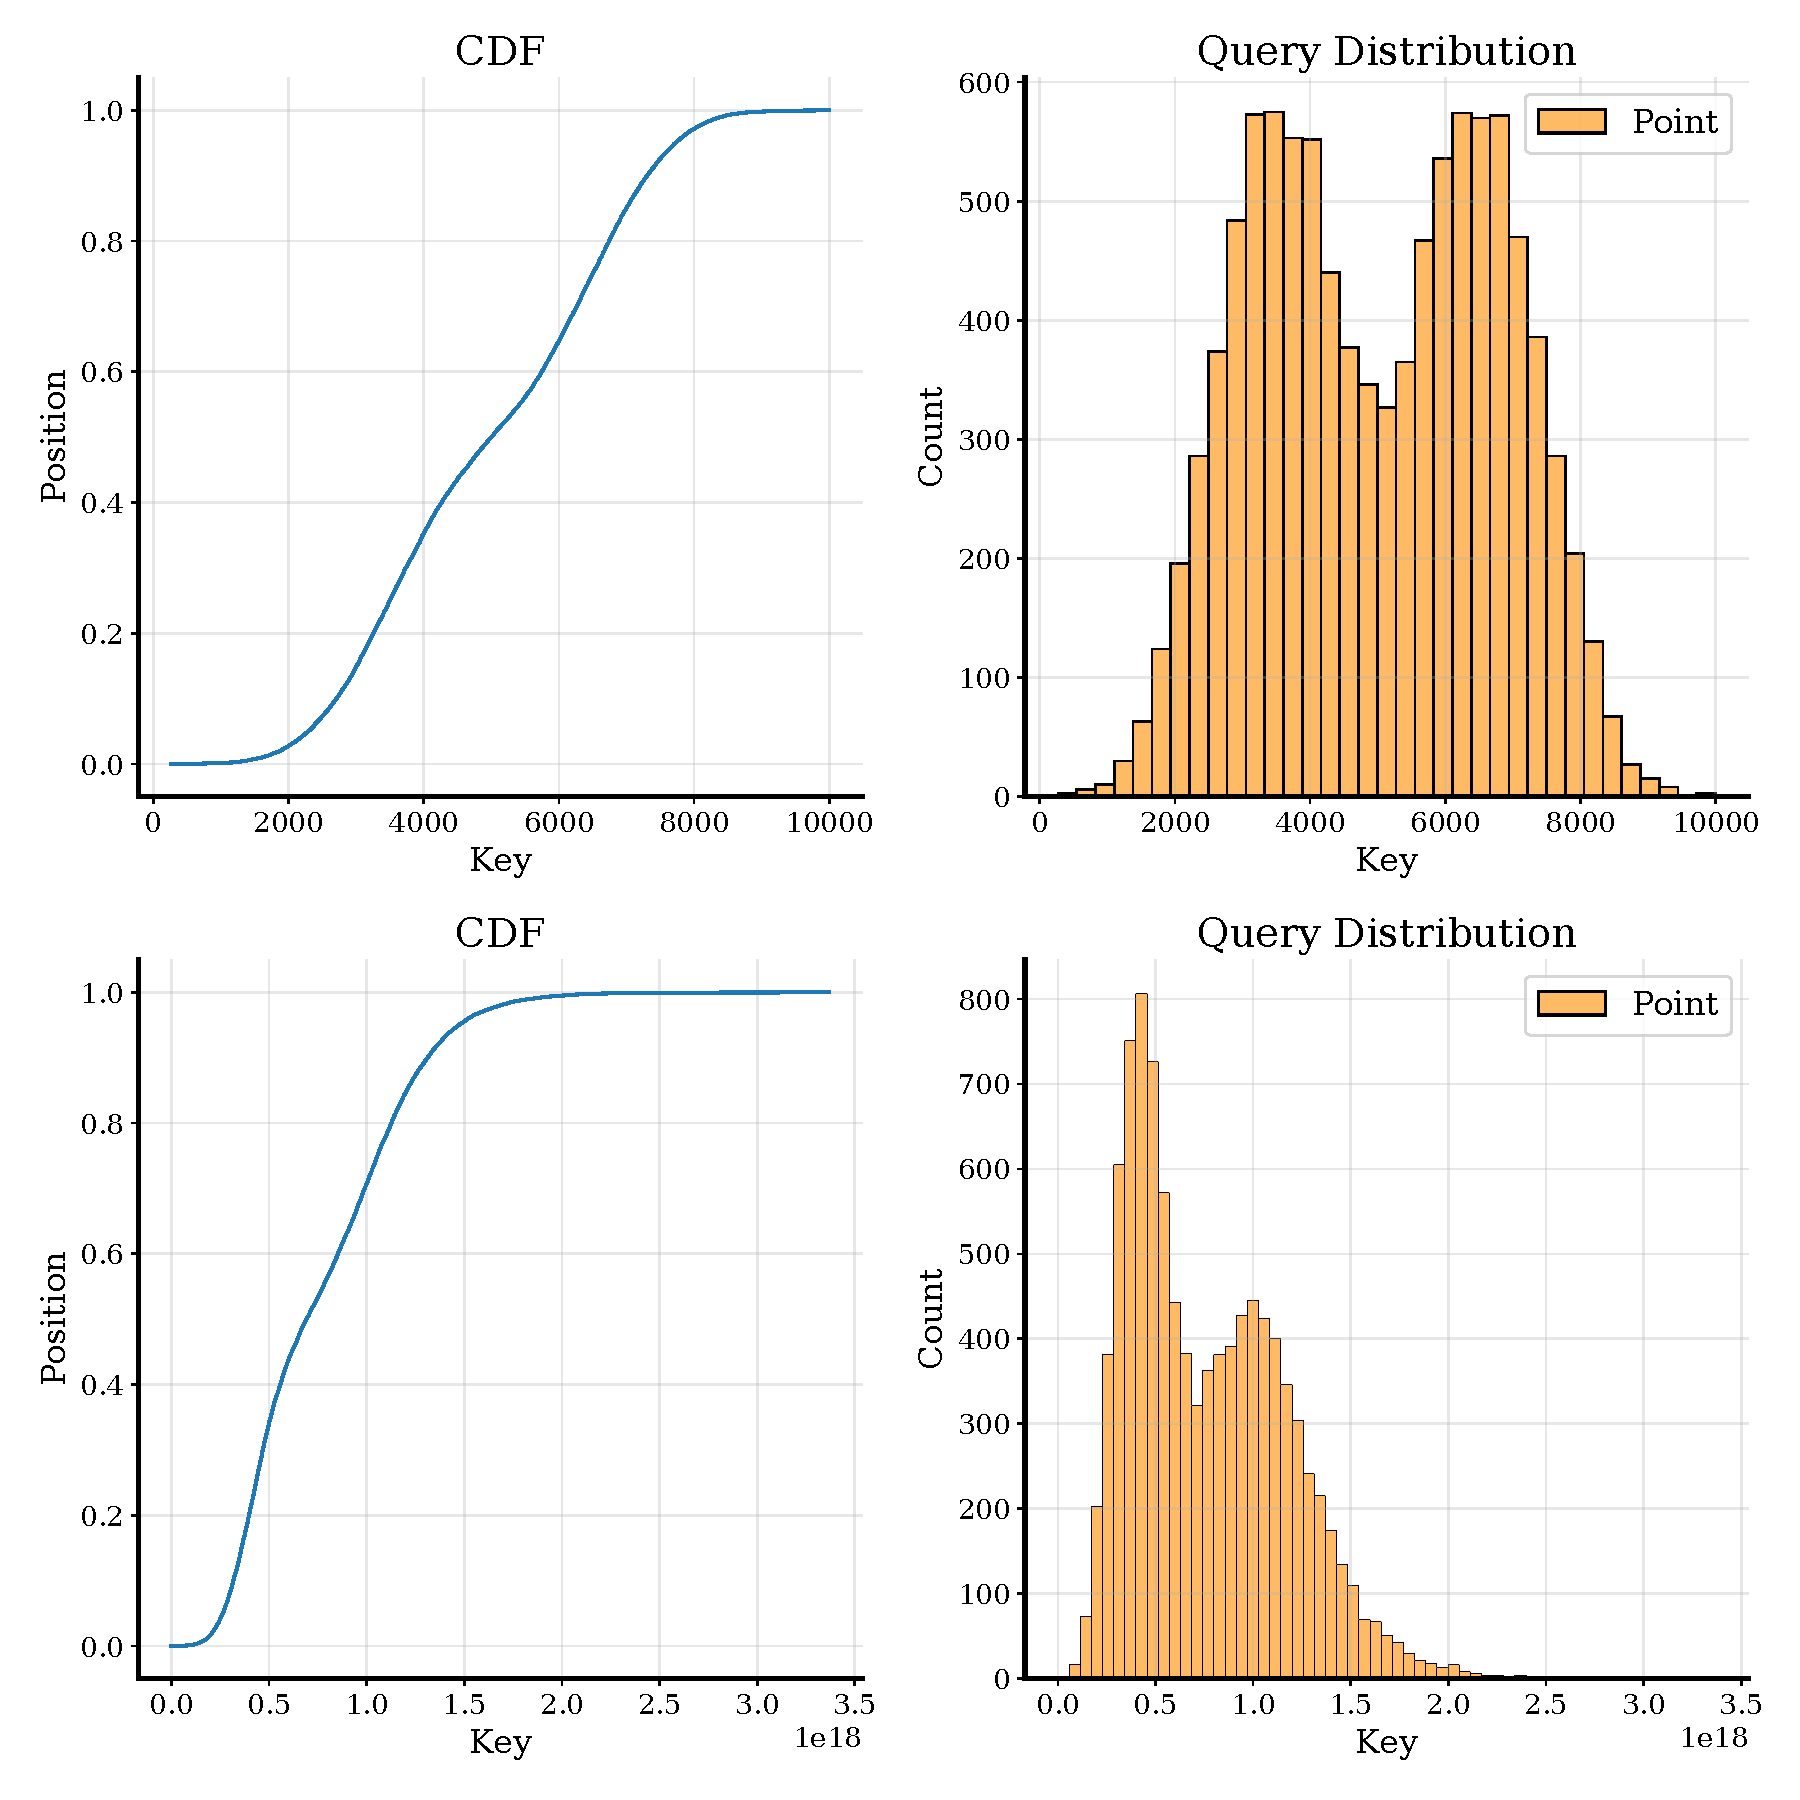
\includegraphics[width=0.8\textwidth]{figures/bimodal.pdf}
    \caption{CDF and Query Distribution of a bimodal worklaod on uniformly and exponentially distributed data}
    \label{fig:bimodal}
\end{figure}


\section{Role of Partitioning Parameters}\label{sec:respartitions}
\begin{itemize}
    \item $$window_size$$, delta for frequency
    \item $$window_size$$ for purity (as of yet)
\end{itemize}

\section{Lookup Performance}\label{sec:resperformance}

\subsection{Frequency Algorithm}

\subsection{Purity Algorithm}

\paragraph{Clear cuts experiment}

First of all, we conducted a rather simple experiment that was designed to confirm the result of \citeauthor{Dittrich2021} \cite{Dittrich2021}. While they hand crafted the boundaries, the partitions for the experiment here were generated by the purity partitioning algorithm. The workload that was executed on the data was split into three regions: the first 10 percent of the keys, the next 75 percent and finally the remaining 15 percent. The first region received 20 percent of the total queries as point queries, the second region received 10 percent of the queries as point queries and 20 percent as range queries. The final region received the remaining 50 percent of queries as point queries. For our experiment, we used 2 million queries in total of which 1 million served as a train workload and 1 million as a test workload. For the benchmarking on the test workload we therefore had the queries depicted in Table \ref{tab:poc_wkl}.

\begin{table}[H]
\centering
\begin{tabular}{rrrrr}
\hline
Region & from & to   & number queries & query type \\ \hline
1      & 0    & 0.1  & 200k           & Point      \\
2      & 0.1  & 0.85 & 100k           & Point      \\
2      & 0.1  & 0.85 & 200k           & Range      \\
3      & 0.85 & 1    & 500k           & Point      \\ \hline
\end{tabular}
\caption{Query Distribution for clear cuts experiment}
\label{tab:poc_wkl}
\end{table}

\begin{figure}[H]
    \centering
    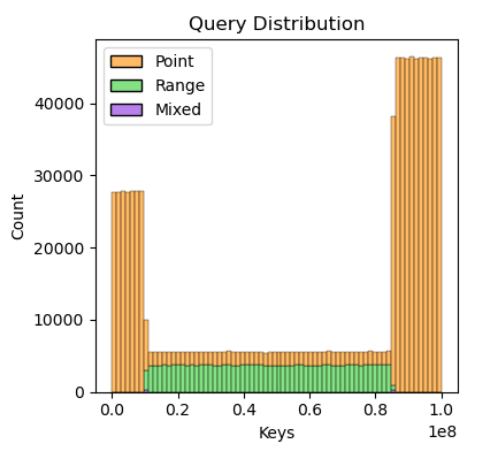
\includegraphics[width=0.6\textwidth]{figures/poc_dist.png}
    \caption{Query Distribution of clear cuts experiment over 100 million uniform dense keys}
    \label{fig:poc_dist}
\end{figure}

The resulting query distribution is visualized in Figure \ref{fig:poc_dist}. As we could already tell from the description of the query distribution, we have two very clear boundaries when looking at frequency as well as purity. While the first and last region are only requested by point queries, we can see that the middle part receives both types of queries. Notably, we see mostly orange and green bars in the figure in this region, as this range contains 75 million keys, but receives only 300 thousand queries. While there is some overlap of these queries, it is rather unlikely that one key from this range is selected for both point and range queries. This overlap would result in a purple bar in the figure. Nevertheless, a generalizing partitioning algorithm should recognize the boundaries and create three partitions accordingly.


//TODO: too small, make this bigger, maybe split single plots
\begin{figure}
    \centering
    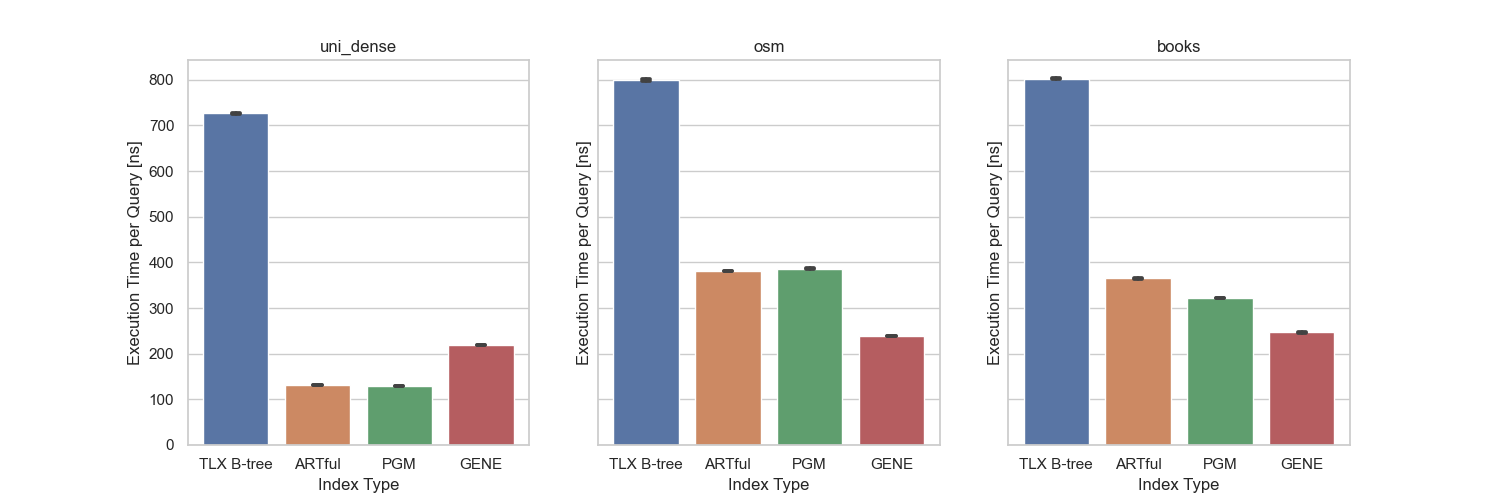
\includegraphics[width=\textwidth]{figures/poc_times.png}
    \caption{Average Query Execution Time on uniform dense data and the osm and books dataset}
    \label{fig:poc_times}
\end{figure}

